% !TeX root = ..\protokoll.tex
\documentclass[../protokoll.tex]{subfiles}
\graphicspath{{\subfix{../images/}}}
\begin{document}
\part{Theorie}
\section{Beugungsbild eines Spaltes im Fernfeld (Fraunhofer-Beugung)}
Hier wird die Abbildung \ref{Theorie 1} betrachtet, wobei D als die Breite des Aufbaus angesehen wird welcher sich in y-Richtung befindet und in x-Richtung ausgedehnt wird. 
\begin{figure}[H]
    \centering
    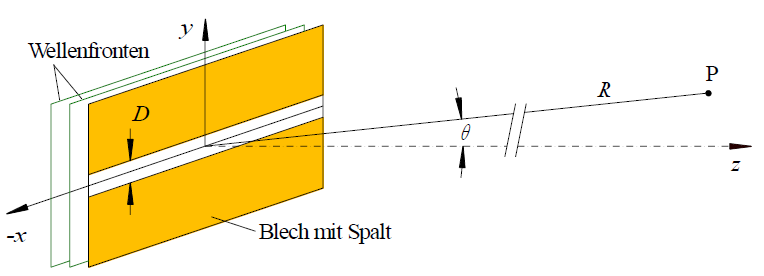
\includegraphics[width=0.6\textwidth]{2023-05-15 - V5 - FRAUNHOFER- und FRESNEL-Beugung, Interferenz/images/Theorie/Blech mit Spalt.png}
    \caption{Beugung an einem Spalt theoretischer Aufbau [entnommen aus dem skript]}
    \label{Theorie 1}
\end{figure}
\end{document}